\chapter{Introduction}
\label{ch:introduction}

\begin{marginfigure}[0.8cm]
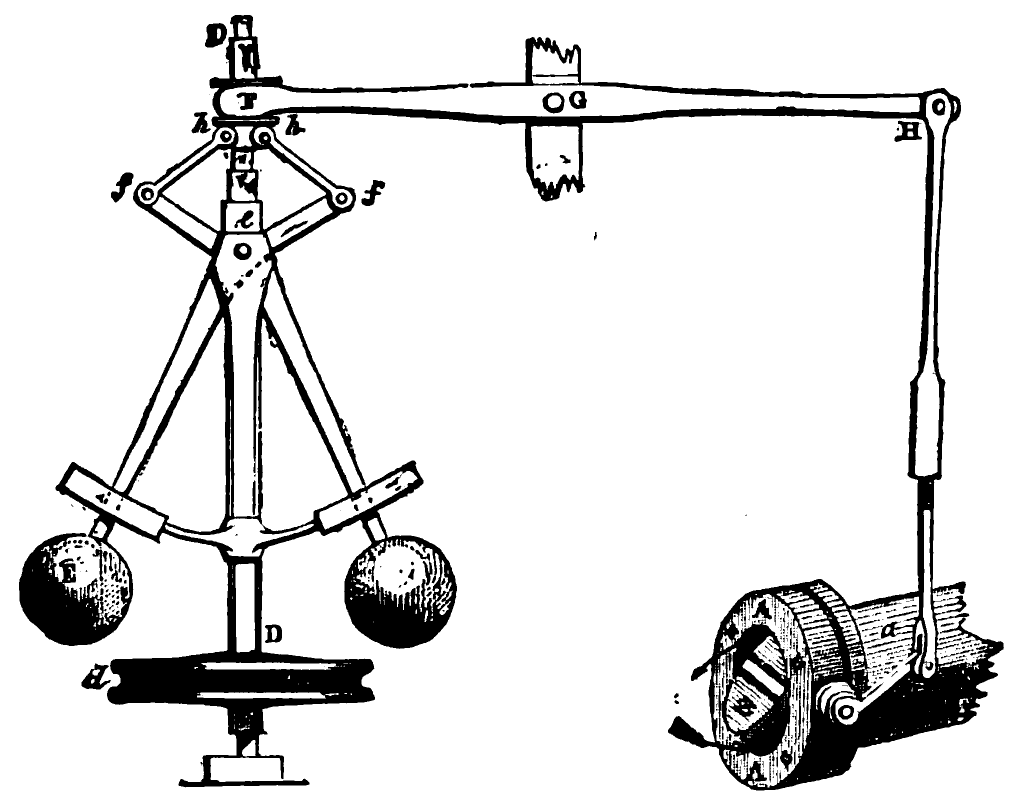
\includegraphics[width=\columnwidth]{img/Centrifugal_governor.png}%
\caption[Centrifugal governor with steam valve.]{Centrifugal governor with steam
valve. Image from \citenum{Routledge:1900:Discoveries}.}
\label{fig:centrifugal-governor}
\end{marginfigure}

\margincite{Routledge:1900:Discoveries}

\lettrine{F}{eedback control} is one of the key enabling technologies of our
time. It is hidden in many devices and appliances without most users even
noticing. The use of feedback controllers dates back to the ancient Greece,
where they were used to control water-based clocks.\ \cite[\ts
II.1]{Mayr:1970:Origins}\iss In the modern world, one of the first uses of
feedback controllers were centrifugal governors \cite{Maxwell:1867:Governors}
(Figure~\ref{fig:centrifugal-governor}) to control steam engines---sparking
the industrial revolution. Since then, feedback controllers have found their
way into our lives and we are using them every day.

A typical example is electronic stability control (ESC) in modern cars,
where the steering angle is constantly measured as a proxy to the driver's
steering intention. Also the turn rate of the car is measured with a gyroscope.
In the case of fading tire grip, the measured turn rate deviates from the
driver's intention. This discrepancy is picked up by the controller and then fed
back as control inputs in the form of brake signals for the individual wheels.
This way the car stays safely on the road, while without feedback control it
would have departed from the road.

While there exist simple model-free feedback methods to compensate deviations
from the desired value, many advanced methods require a mathematical model of
the controlled system. The model predicts the state evolution of the system and
can be used to either synthesize the feedback law or to calculate the feedback
signal in each time step. Model-based control usually requires less tuning and
can have advanced features like lookahead for reference tracking. Since we want
to make use of such features, the controllers in this thesis are all
model-based.

The classic way of doing model identification is physical modeling, e.g.,
Newton's laws can be used to deduce the mathematical equations of motion of
mechanical systems. If physical modeling is not possible, either due to the lack
of knowledge about the system, or because precise enough measurements can not be
made, \emph{system identification}~\cite{Ljung:1999:System} is often used to
find an approximation to the dynamics.

For some applications, building a controller a priori is not viable. The
systems in question might not be known beforehand or can be subject to changes
in the dynamics. In these cases, offline system identification can lead to bad
\margincite{Kumar.Varaiya:1986:Stochastic}%
system performance or may not be able to achieve the desired controller
requirements. \emph{Adaptive control}~\citenum{Kumar.Varaiya:1986:Stochastic}
offers the possibility to create controllers that are able to adapt to unknown
plants, changing plant dynamics, or unknown environments. Adaptivity means that
the control system needs a way of learning about the relevant dynamics of the
plant or the environment.

\subsection*{Disturbance Forecasting}

For many applications, controllers are built for feedback-based disturbance
rejection, which means that the effect of outside disturbances is kept small by
using the measured tracking error. However, sometimes feedback-based
disturbance rejection is not fast enough due to high performance demand or slow
measurement processes. In such cases it can help to incorporate a prediction of
the disturbance to eliminate parts of the error introduced by the disturbance in
advance.

General time-series forecasting is a challenging topic, but it gets more
manageable if the disturbance in question is of periodic nature---for example
when the origin of the disturbance is tied to the day-night-cycle or periodic
motions. In such cases, the use of periodic models to predict the disturbances
can considerably increase predictive performance and, thus, make the use of
disturbance forecasting much more available.

\subsection*{Active Identification}

Most adaptive control methods only learn in a passive manner. The available
information is used, but it is not attempted to invest control energy for
exploration or identification. In episodic settings, where the control system
executes the same task multiple times, this is often sufficient. However, for
non-episodic problems---the control of a single trial---active exploration is
an important aspect. When a system never runs twice under the same conditions,
it is crucial not only to use the available information in the best possible
way, but also to actuate the system such that the relevant information is
generated. This simultaneous identification and control is the realm of
\emph{dual control}~\cite{Wittenmark:1995:Adaptive}.

The key to differentiate between these methods is the time at which the
information is acquired. In system identification, the data is collected
upfront, before the controller is used on the plant. This also means that the
controller is not updated online. An adaptive controller is learning
``on-the-fly'', while the system is running. It collects data and updates the
internal model regularly. A dual control system goes one step further and uses
reasoning about the learning process itself to find the optimal actions. This
means that a dual controller incorporates the predicted future information
acquisition into the decision process.

\section*{Outline}

Part~\ref{par:prelimininaries} introduces the relevant mathematical background.
Gaussian process regression (Chapter~\ref{ch:gaussian-processes}) is used to
model system dynamics and external error sources. Model predictive control
(Chapter~\ref{ch:discrete-time-optimal-control}) is a well-suited control
framework for incorporating predictions into the control system. We also give
an overview on the field of adaptive control
(Chapter~\ref{ch:adaptive-control}).

Part~\ref{par:predictive-disturbance-control} shows how quasiperiodic Gaussian
process models can be used to enhance control performance. The general concept
of quasiperiodic disturbance forecasting in combination with reference tracking
model predictive control is introduced
(Chapter~\ref{ch:periodic-error-correction}) and subsequently applied to an
experimental problem in astronomical imaging: the periodic error correction in
telescope guiding (Chapter~\ref{ch:predictive-error-correction-for-telescopes}).
Based on this work, we developed software to use the periodic error correction
feature in an open source telescope guiding system
(Chapter~\ref{ch:software-implementation-phd-guiding}).

Part~\ref{par:dual-control} is concerned with the concept and application of
dual control to nonlinear systems. We first give a general overview of the dual
control literature and a classic algorithm
(Chapter~\ref{ch:introduction-to-dual-control}) which is then extended
to modern nonlinear regression techniques
(Chapter~\ref{ch:nonlinear-extensions-to-dual-control}). We further extend this
nonlinear framework to constrained systems with linear cost structure
and show a potential application to building control
(Chapter~\ref{ch:dual-control-for-buildings}).

Chapter~\ref{ch:conclusions} gives a concise summary of the work
presented in this thesis and concludes with an outlook on future research
directions.

\section*{Publications}

{\setlength{\parindent}{0pt}

Parts of the work in this thesis were done in collaboration with colleagues
and are based on the following publications:

\vspace{5mm}

Chapters~\ref{ch:periodic-error-correction} and
\ref{ch:predictive-error-correction-for-telescopes} are based on the
following journal publication:

\printpublication{Klenske.ea:2016:Gaussian}

A conference version was published in:

\printpublication{Klenske.Zeilinger.ea:2013:Nonparametric}

Chapters~\ref{ch:introduction-to-dual-control} and
\ref{ch:nonlinear-extensions-to-dual-control}, as well as
Section~\ref{sec:sparse-spectrum-approximation}, are based on the following
journal publication:

\printpublication{Klenske.Hennig:2015:Dual}

Chapter~\ref{ch:dual-control-for-buildings} is based on the following conference
publication:

\printpublication{Klenske.Hennig.ea:2016:Approximate}
}
